\documentclass[a4paper,11pt]{report}

\usepackage{fancyhdr}
\usepackage{graphicx}
\usepackage[top=1.5cm, bottom=3cm, left=2.5cm, right=2.5cm]{geometry} % Adjust margins
\usepackage{setspace}
\usepackage[linktoc=page]{hyperref}
\usepackage{sectsty}
\chapterfont{\centering}
\usepackage{makeidx}
\usepackage{url}
\usepackage[square,sort,comma,numbers]{natbib}
\usepackage{framed}
\usepackage{longtable}
\usepackage{amsfonts}
\usepackage{amsmath}
\usepackage{booktabs} % For better looking tables
\usepackage{array} 
\usepackage[noend,ruled,noline,linesnumbered,algochapter]{algorithm2e}

% Set header and footer space
\setlength{\headheight}{0pt} % Remove extra height in header
\setlength{\headsep}{0.5cm} % Reduce space between header and text

% Title Page
\begin{document}

% Fancy header and footer settings
\pagestyle{fancy}
\fancypagestyle{plain}{%
    \fancyhf{} % clear all header and footer fields
    \renewcommand{\headrulewidth}{0pt}
    \fancyfoot[L]{\textit{©Daffodil International University}}
    \fancyfoot[R]{\thepage}
}

\fancyhf{} % clear all header and footer fields
\renewcommand{\headrulewidth}{0pt}
\fancyfoot[L]{\textit{©Daffodil International University}}
\fancyfoot[R]{\thepage}

% Set headers: chapter on the left, section on the right
\fancyhead[L]{\nouppercase{\leftmark}} % Chapter title on the left
\fancyhead[R]{\nouppercase{\rightmark}} % Section title on the right

% Title Page
\begin{titlepage}

\vspace*{2cm} % Adjust this value to increase the header space

\begin{center}
{\huge\bf Title of Your Mini Lab Project}
\end{center}

\vspace{2cm}

\begin{center}
\Large \bf Submitted By
\end{center}

\vspace{.1cm}

\begin{table}[h!]
\centering
\begin{tabular}{|c|c|}
\hline
\textbf{      Student Name      } & \textbf{  Student ID  } \\
\hline
Student-1 Name & Student-1 ID \\
\hline
Student-2 Name & Student-2 ID \\
\hline
Student-3 Name & Student-3 ID \\
\hline
Student-4 Name & Student-4 ID \\
\hline
Student-5 Name & Student-5 ID \\
\hline
\end{tabular}
\end{table}

\vspace{2cm}

\begin{center}
{\Large\bf MINI LAB PROJECT REPORT}\\
\vspace{0.2cm}
\Large This Report Presented in Partial Fulfillment of the course  \textbf{CSEXXX: Subject Name in the Computer Science and Engineering Department}
\end{center}

\vspace{2cm}

\begin{center}

\includegraphics[scale=0.5]{./figures/DIU Logo}
\end{center}

\begin{center}
	\Large\textbf{DAFFODIL INTERNATIONAL UNIVERSITY}\\
 \textbf{\textsc{Dhaka, Bangladesh}}
\end{center}

\begin{center}
\textbf{\today}
\end{center}

\end{titlepage}

\clearpage

% Set Roman page numbering for initial pages
\pagenumbering{roman}
\setcounter{page}{1}

% Declaration-------------------------
\phantomsection

\vspace*{1.5cm} 

\addcontentsline{toc}{chapter}{Declaration}

\begin{center}
    {\LARGE \textbf{DECLARATION}}\\
   % \line(1,0){430}
\end{center}

\onehalfspacing

\noindent We hereby declare that this lab project has been done by us under the supervision of \textbf{Name of the course teacher}, \textbf{course teacher's Designation}, Department of Computer Science and Engineering, Daffodil International University. We also declare that neither this project nor any part of this project has been submitted elsewhere as lab projects. 

\vspace{.8cm}

\noindent \textbf{Submitted To:} \\[1cm]

\noindent\rule{6cm}{0.4pt}\\
\textbf{Course Teacher's Name} \\
Designation \\
Department of Computer Science and Engineering \\
Daffodil International University \\

\vspace{.5cm}

% Table
\begin{center}
    \textbf{Submitted by}
\end{center}

\vspace{.2cm}

\begin{table}[h!]
\centering
\renewcommand{\arraystretch}{3} % Increase row height for more space
\setlength{\tabcolsep}{10pt} % Adjust column spacing

\begin{tabular}{|p{0.48\textwidth}|p{0.35\textwidth}|} % Equal column widths

\hline
\multicolumn{2}{|c|}{
    \begin{minipage}{\linewidth}
        \centering
        \vspace{1.5cm} % Space above the name for signature
        \rule{6cm}{0.4pt} % Signature line
        \\
        \textbf{Student Name} \\ Student ID: \\ Dept. of CSE, DIU
    \end{minipage}
} \\
\hline

\begin{minipage}{\linewidth}
    \centering
    \vspace{1.5cm} % Space above the name for signature
    \rule{6cm}{0.4pt} % Signature line
    \\
    \textbf{Student Name} \\ Student ID: \\ Dept. of CSE, DIU
\end{minipage} &

\begin{minipage}{\linewidth}
    \centering
    \vspace{1.5cm} % Space above the name for signature
    \rule{6cm}{0.4pt} % Signature line
    \\
    \textbf{Student Name} \\ Student ID: \\ Dept. of CSE, DIU
\end{minipage} \\
\hline

\begin{minipage}{\linewidth}
    \centering
    \vspace{1.5cm} % Space above the name for signature
    \rule{6cm}{0.4pt} % Signature line
    \\
    \textbf{Student Name} \\ Student ID: \\ Dept. of CSE, DIU
\end{minipage} &

\begin{minipage}{\linewidth}
    \centering
    \vspace{1.5cm} % Space above the name for signature
    \rule{6cm}{0.4pt} % Signature line
    \\
    \textbf{Student Name} \\ Student ID: \\ Dept. of CSE, DIU
\end{minipage} \\
\hline

\end{tabular}

\end{table}


\newpage
%Abstract
\phantomsection
\vspace*{1.5cm} 
\addcontentsline{toc}{chapter}{Course \& Program Outcome}
\setlength{\headheight}{14pt}
\begin{center}
	{\LARGE \bf COURSE \& PROGRAM OUTCOME}\\
	%\line(1,0){430}
\vspace*{1.5cm} 
\begin{flushleft}
The following course have course outcomes as following:.
\end{flushleft}

% table of CO's....................
\begin{table}[h!]
\centering
\caption{Course Outcome Statements}
\vspace{0.1cm} % Adds a 0.5 cm space between the caption and the table
\begin{tabular}{|p{0.06\textwidth}|p{.9\textwidth}|}
\hline
\textbf{CO's} & \textbf{Statements} \\
\hline
CO1 & \textbf{Define} and \textbf{Relate} classes, objects, members of the class, and relationships among them needed for solving specific problems \\
\hline
CO2 & \textbf{Formulate} knowledge of object-oriented programming and Java in problem solving \\
\hline
CO3 & \textbf{Analyze} Unified Modeling Language (UML) models to \textbf{Present} a specific problem \\
\hline
CO4 & \textbf{Develop} solutions for real-world complex problems \textbf{applying} OOP concepts while evaluating their effectiveness based on industry standards. \\
\hline
\end{tabular}
\end{table}

\vspace{1cm}
%----------------------------
% table for Mapping of CO, PO, Blooms, KP and CEP---------
\begin{table}[h!]
\centering
\caption{Mapping of CO, PO, Blooms, KP and CEP}
\begin{tabular}{|>{\centering\arraybackslash}m{2cm}|>{\centering\arraybackslash}m{2cm}|>{\centering\arraybackslash}m{2cm}|>{\centering\arraybackslash}m{2cm}|>{\centering\arraybackslash}m{2cm}|}
\hline
\textbf{CO} & \textbf{PO} & \textbf{Blooms} & \textbf{KP} & \textbf{CEP} \\
\hline
CO1 & PO1 & C1, C2 & KP3 & EP1,EP3 \\
\hline
CO2 & PO2 & C2 & KP3 & EP1,EP3 \\
\hline
CO3 & PO3 & C4, A1 & KP3 &EP1,EP2 \\
\hline
CO4 & PO3 & C3, C6, A3, P3 & KP4 & EP1,EP3 \\
\hline
\end{tabular}
\end{table}
\begin{flushleft}
The mapping justification of this table is provided in section \textbf{4.3.1}, \textbf{4.3.2} and \textbf{4.3.3}.
\end{flushleft}



\setlength
{\headheight}{12pt}


% Table of contents
\renewcommand*\contentsname{Table of Contents}
\tableofcontents
\clearpage

\renewcommand\bibname{References}
\clearpage

% Start of report and chapters
\pagenumbering{arabic} % Switch to Arabic numbering
\setcounter{page}{1}

% Reapply header and footer settings for the main content
\fancyhf{} % clear header and footer
\fancyfoot[L]{\textit{©Daffodil International University}}
\fancyfoot[R]{\thepage}
\fancyhead[L]{\nouppercase{\leftmark}} % Chapter title on the left
\fancyhead[R]{\nouppercase{\rightmark}} % Section title on the right

% Chapters content...................................
\chapter{Introduction}

%This is for reference only. Delete before finalization
\begin{center}
\noindent Every chapter should start with 1-2 sentences on the outline of the chapter.
\end{center}
%This is for reference only. Delete before finalization


% Start sections and sub-sections
\begin{flushleft}
\section{Introduction}
This section should present the background and a problem statement that your project aims to solve.

\section{Motivation}
The computational motivation that encourages you to solve the problem should be stated here clearly. In addition, you can mention why solving this problem will benefit you.

\section{Objectives}
Enumerate the objectives in clear and specific terms.


\section{Feasibility Study}
Put a summary of similar research study, case study, methodological contribution of existing projects, web applications, and mobile apps similar to your work \cite{kleinberg2006algorithm}.

\section{Gap Analysis}
Here summaries the gap where you intend to work.

\section{Project Outcome}
What are or could be the possible outcomes of your work?
\end{flushleft}
\chapter{Proposed Methodology/Architecture}

%This is for reference only. Delete before finalization
\begin{center}


Every chapter should start with 1-2 sentences on the outline of the chapter.
    
\end{center}
%This is for reference only. Delete before finalization

\begin{flushleft}
\section{Requirement Analysis \& Design Specification}
\subsection{Overview}
\subsection{Proposed Methodology/ System Design}

\begin{figure}[h] % 'h' for placing it "here"
    \centering
    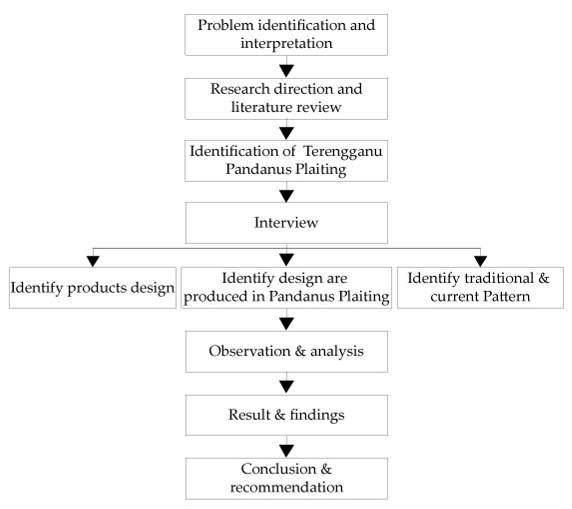
\includegraphics[width=0.5\textwidth]{figures/flowdiagram.png} % Replace 'diagram.png' with your image file
    \caption{This is a sample diagram}
    \label{fig:sample}
\end{figure}

\subsection{UI Design}

\section{Overall Project Plan}

\end{flushleft}
\chapter{Implementation and Results}

Every chapter should start with 1-2 sentences on the outline of the chapter.
\end{center}

%This is for reference only. Delete before finalization

\section{Implementation}
\section{Performance Analysis}
\section{Results and Discussion}

\chapter{Engineering Standards and Mapping}


Every chapter should start with 1-2 sentences on the outline of the chapter.
\end{center}
%This is for reference only. Delete before finalization

\section{Impact on Society, Environment and Sustainability}
\subsection{Impact on Life}
\subsection{Impact on Society \& Environment}
\subsection{Ethical Aspects}
\subsection{Sustainability Plan}


%\section

\section{Project Management and Team Work}
Provide a cost analysis in terms of budget required and revenue model. In case of budget, you must show an alternate budget and rationales. 

\section{Complex Engineering Problem}

\subsection{Mapping of Program Outcome} 

In this section, provide a mapping of the problem and provided solution with targeted Program Outcomes (PO's).

\begin{center}
    \begin{table}[ht]
        \centering
        \caption{Justification of Program Outcomes}
        \begin{tabular}{|p{0.2\textwidth}|p{0.7\textwidth}|}
            \hline
            \textbf{PO's} & \textbf{Justification} \\
            \hline
            PO1 & Justification of PO1 attainment \\
            \hline
            PO2 & Justification of PO2 attainment \\
            \hline
            PO3 & Justification of PO3 attainment \\
            \hline
        \end{tabular}
        \label{tab:po_justification}
    \end{table}
\end{center}



\subsection{Complex Problem Solving} 
In this section, provide a mapping with problem solving categories. For each mapping add subsections to put rationale (Use Table~\ref{tab:p_solve}). For P1, you need to put another mapping with Knowledge profile and rational thereof.
\begin{center}
    \begin{table}[ht]
        \centering
        \caption{Mapping with complex problem solving.}
        \begin{tabular}{|p{0.12\textwidth}|p{0.12\textwidth}|p{0.12\textwidth}|p{0.12\textwidth}|p{0.12\textwidth}|p{0.12\textwidth}|p{0.12\textwidth}|}
        \hline
        EP1& EP2& EP3& EP4& EP5& EP6& EP7\\
        Dept of Knowledge & Range of Conflicting Requirements & Depth of Analysis & Familiarity of Issues & Extent of Applicable Codes & Extent of Stakeholder Involvement & Inter-dependence\\
        \hline 
        $\sqrt{}$ & $\sqrt{}$ &&&&&\\
        &&&&&&\\
        \hline 
        \end{tabular}
        \label{tab:p_solve}
    \end{table}
\end{center}


\subsection{Engineering Activities}
In this section, provide a mapping with engineering activities. For each mapping add subsections to put rationale (Use Table~\ref{tab:e_act}).
\begin{center}
    \begin{table}[ht]
        \centering
                \caption{Mapping with complex engineering activities.}
        \begin{tabular}{|p{0.18\textwidth}|p{0.18\textwidth}|p{0.18\textwidth}|p{0.18\textwidth}|p{0.18\textwidth}|}
        \hline
        EA1& EA2& EA3& EA4& EA5\\
        Range of resources & Level of Interaction & Innovation & Consequences for society and environment & Familiarity\\
        \hline 
        $\sqrt{}$ & $\sqrt{}$ &&&\\
        &&&&\\
        \hline 
        \end{tabular}
        \label{tab:e_act}
    \end{table}
\end{center}

\chapter{Conclusion}

%This is for reference only. Delete before finalization
\begin{center}
Every chapter should start with 1-2 sentences on the outline of the chapter.
\end{center}
%This is for reference only. Delete before finalization

\section{Summary}
\section{Limitation}
\section{Future Work}


% References section
\renewcommand\bibname{References} % Ensure "References" title
\addcontentsline{toc}{chapter}{References} % Add "References" to TOC
\bibliographystyle{unsrt}
\bibliography{fydp} % Make sure fydp.bib exists in the same directory

\clearpage

\end{document}
